\documentclass[11pt]{ctexart}
\usepackage{a4}
\usepackage{graphicx}
\usepackage{geometry}
\geometry{a4paper,left=2cm,right=2cm,top=2.5cm,bottom=2.5cm}

\title{几何基础作业2}
\author{无名}
\date{\today}

\begin{document}
\maketitle

\section{《原本》第一卷叙述证明三条高线交于一点}
\begin{center}
    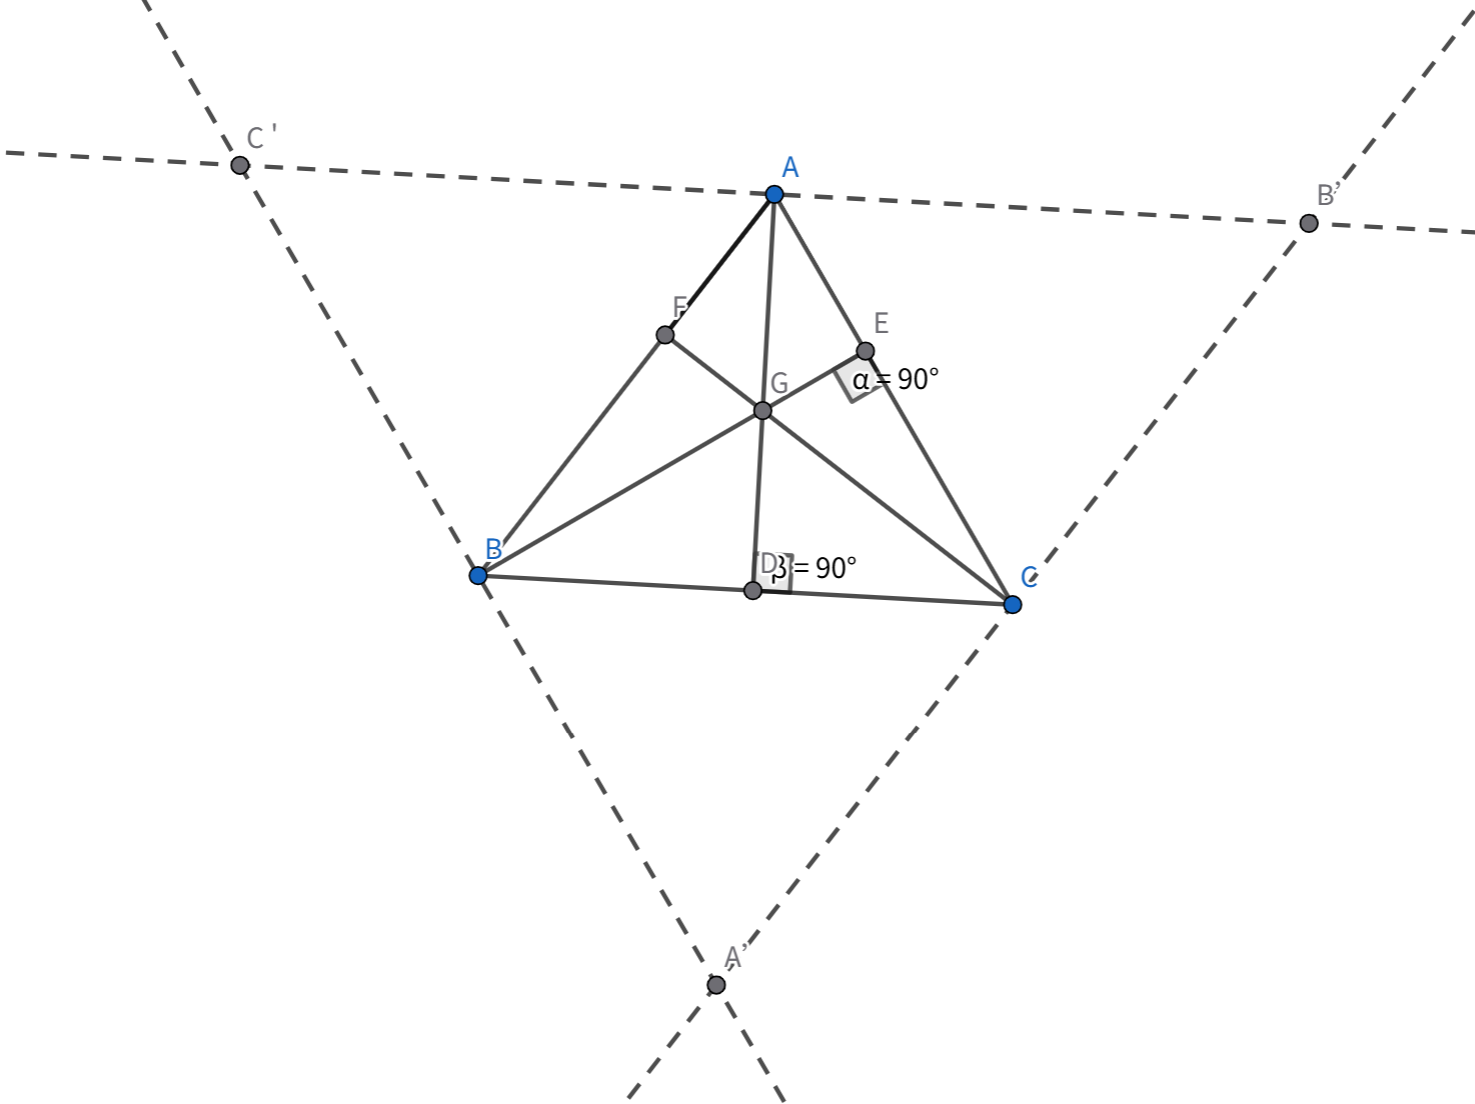
\includegraphics[width=0.7\linewidth]{01.png}
\end{center}

如图，已知有$\bigtriangleup ABC$，现作$AD\bot BC$于D，$BE\bot AC$于E（命题12）使得AD，BE交于G，连接CG延长交AB于F，则需证明$CF\perp AB$。

过A作BC平行线$l_A$，过B做AC平行线$l_B$，过C做AB平行线$l_C$（命题31），记$l_Al_B$交于C'，$l_Bl_C$交于A'，$l_Al_C$交于B'。

此时由于$AC//BA'$，则$\angle BA'C =\angle ACB'$,
由于$AC//BC',BC//AC'$，则$\angle B'AC=\angle AC'B=\angle CBA'$ （命题29）

由于$AC//BA',AB//CA'$,$ABA'C$构成了一个平行四边形，则有$AC=BA'$（命题31）

故$\bigtriangleup ACB' \cong \bigtriangleup BA'C$(命题26)

同理$\bigtriangleup BCA' \cong \bigtriangleup C'AB$,即$\bigtriangleup C'AB \cong \bigtriangleup BCA' \cong \bigtriangleup AB'C$

故有$C'A=AB'$，即A为B'C'的中点。同理，BC均为C'A',A'B'中点。

由于平行，显然$AD\bot B'C'$，故对于$\bigtriangleup C'AG和\bigtriangleup B'AG$，有$\bigtriangleup B'AG \cong \bigtriangleup C'AG$(命题26)，进而得到$C'G=B'G$

由$\bigtriangleup C'BG和\bigtriangleup A'BG$的关系可以得到$A'G=B'G=C'G$

由于三边相等，$\bigtriangleup A'CG\cong \bigtriangleup B'CG$(命题26)，进而$\angle A'CG= \angle B'CG$，故$\angle A'CG= \angle B'CG$均为直角(命题13)

进而$AB\bot CF$,CF也是高线，三个高线交于一点。
\section{叙述证明阿基米德折弦定理}

阿基米德折弦定理:在圆中，若由两条不等长弦组成的折弦所对弧中点在较长弦上的垂足，即为折弦的中点
\begin{center}
    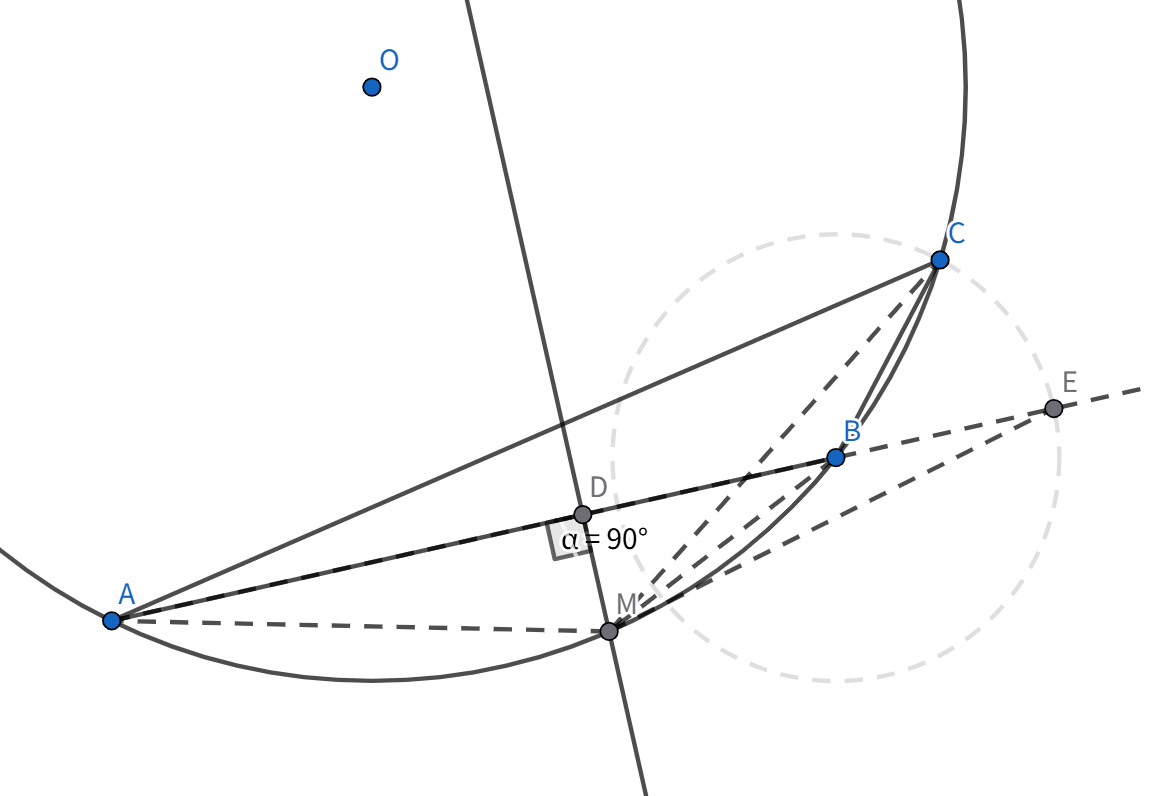
\includegraphics[width=0.8\linewidth]{02.png}
\end{center}

如图，AB,BC是圆弧的两条弦，$AB>BC$,M是圆弧ABC的中点，M向AB做垂线于D，则D是折线ABC的中点，即$AD=DB+BC$

证明:

延长AB，使得$BE=BC$，连接各点。即需要证明$AD=DE$

M是圆弧ABC的中点，意味着$AM=MC,\angle MAC=\angle MCA=\angle MBA$

AMBC四点共圆，则$\angle CBM+\angle CAM =\pi$

则$\angle ABM+\angle CAM =\pi$

由于$\angle ABM+\angle EBM =\pi$

则$\angle CBM=\angle EBM$，同时$BC=BE$可得到$\bigtriangleup CBM \cong \bigtriangleup EBM$

从而$ME=MC=AM$

由于$MD\bot AE$，则$AD=DE$，从而得证
\end{document}